
Differential gene expression (DE) refers to the difference in the gene expression between two or more varieties based on read counts from replicated samples. An approach for comparing gene expression levels between replicated conditions of RNA sequencing data replies on counting reads that map to features of insterest. Within such count-based methods, many flexible and advanced statistical approaches now exist and offer the ability to adjust for covariates (e.g., batch effects) \citep{zhou2014robustly}. Often, these methods include some sort of sharing of information across features to improve inferences in small samples. Niemi et al. developed a hierarchical negative binomial model and drew inferences using a computationally tractable empirical Bayes approach to inference \citep{niemi2015empirical}. In this report, I modified Niemi's method, applied it to DE analysis context, and compared it to five alternative methods ({\tt edgeR, DESeq, DESeq2, EBSeq, sSeq}) via a simulation study based on a maize experiment. This article has supplementary material online \href{https://github.com/xiyuansun/kellycc}{GitHub repo for this creative component report} 





\chapter{METHOD}

\section{Estimating the difference between read counts for a given gene}

To detemine whether the read count differences between different conditions for a given gene are greater than expected by chance, differential gene expression (DGE) tools must find a way to estimate that difference \citep{dundar2015introduction}.The two basic tasks of all DGE tools are: (1) Estimate the magnitude of differential expression between two or more conditions based on read counts from replicated samples, i.e., calculate the fold change of read counts, taking into account the differences in sequencing depth and variability; (2) Estimate the significance of the difference and correct for multiple testing. 

\section{Empirical Bayes identification of gene differential expression from RNA-seq read counts}

I consider an RNA sequencing (RNA-seq) experiment that involves two genetic varieties. For each variety, replicate RNA samples are isolated and assessed for quality. Complementary DNA (cDNA) libraries, consisting of short cDNA fragments derived from RNA, are constructed. Then, next generation sequencing technology is used to determine the {\tt reads}, in the cDNA libraries \citep{niemi2015empirical}. These reads are processed using bioinformatic algorithms to match the reads to genes. The results of read processing are summarized by a gene $\times$ sample matrix of counts. See Datta and Nettleton \citep{datta2014statistical} for more details on RNA-seq experiments and data from a statistical perspective, and see \citep{paschold2012complementation} for the biological background behind the use of RNA-seq to study gene expression differentiation. 

To use RNA-seq counts to identify genes displaing differential expression (DE), I built a hierarchical to borrow information across gene-variety means and across gene-specific overdispersion parameters, estimate the hyperparameters using an empirical Bayes procedure, and calculate empirical Bayes posterior probabilities for DE. 

\subsection{Hierarchical model for RNA-seq counts}

Let $Y_{gij}$ be the count for gene $g=1,2,..., G$, variety $i=1,2$, and replicate $j=1,2,3,...,n_i$.

I assume

\begin{equation}
\label{eq:1}
Y_{gij} \stackrel{ind}{\sim} NB(\exp(\lambda_{gi}+\gamma_{ij}), \exp(\psi_g))
\end{equation}

with mean $\mu_{gij} = \exp{(\lambda_{gi}+\gamma_{ij})}$ and dispersion $\phi_g = \exp{(\psi_g)}$

where $\gamma_{ij}$ terms are normalization factors that account for differencees in the thoroughness of sequencing from sample to sample. 

Following \citep{ji2014estimation}, I reparameterize the gene-variety mean structure into the genespecific average $\beta_{g1}$ and half-variety difference $\beta_{g2}$. For my differential expression study where number of varieties is 2, I let $i=1,2$ indicate the two varieties. The reparameterization is

\begin{equation}
\label{eq:2}
\beta_{g1} = \frac{\lambda_{g1}+\lambda_{g2}}{2}, \beta_{g2} = \frac{\lambda_{g1}-\lambda_{g2}}{2}
\end{equation}

I assume a hierarchical model for the gene-specific mean parameters and overdispersion parameters. Initially, I assume the variety averages, half-variety averages, and overdispersion parameters follow normal distributions

\begin{equation}
\label{eq:3}
\beta_{g1} \stackrel{ind}{\sim} N(\eta_{\beta_1}, \sigma^2_{\beta_1}), \beta_{g2} \stackrel{ind}{\sim} N(\eta_{\beta_2} , \sigma^2_{\beta_2}), \psi_g \stackrel{ind}{\sim} N(\eta_\psi, \sigma^2_\psi)
\end{equation}

The link function is \ref{eq:4}
\begin{equation}
\label{eq:4}
log(\mu_{gij}) = \lambda_{gi} + \gamma_{ij} = x_i^T \beta_g + log(N_{ij})
\end{equation}


\subsection{Empirical Bayes Method}

I categorize the parameters of the model into gene-specific parameters $\theta = (\theta_1, ..., \theta_G)$ where $\theta_g = (\beta_{g1}, \beta_{g2}, \psi_g)$, normalization factors $\gamma = (\gamma_{11}, ..., \gamma_{V n_V})$, and hyperparameters $\pi = (\eta, \sigma)$ where $\eta = (\eta_{\beta_1}, \eta_{\beta_2}, \eta_\psi)$ and $\sigma = (\sigma_{\beta_1}, \sigma_{\beta_2}, \sigma_\psi)$. I obtain estimates for the hyperparameters and then base gene-specific inference on the posterior conditional on these estimates \citep{niemi2015empirical}.

To obtain normalization factors $\hat{\gamma}$, I use the weighted trimmed mean of $M$ values (TMM). I use edgeR to obtain genewise dispersion estimates, $\hat{\psi}_g$, and the generalized linear model methods to obtain estimates for the remaining gene-specific parameters ($\hat{\beta}_{g1}, \hat{\beta}_{g2}$)\citep{robinson2010scaling}. Using $\hat{\theta}_g = (\hat{\beta}_{g1} , \hat{\beta}_{g2}, \hat{\psi}_g)$, I estimate hyperparameters for the location and scale parameters in the hierarchical model using a central method of moments approach. 

Conditional on the estimated normalization factors $\hat{\gamma}$ and hyperparameters $\hat{\pi}$, I perform a Bayesian analysis to re-estimate the gene-specific parameters and describe their uncertainty \citep{niemi2015empirical}. Equation \ref{eq:5} shows that conditional on $\hat{\gamma}$ and $\hat{\pi}$, the gene-specific parameters are independent and therefore conditional posterior inference across the genes can be parallelized. 

\begin{equation}
\label{eq:5}
\begin{split}
& p(\theta | y, \hat{\pi}, \hat{\gamma})  \propto \\ & \prod_{g=1}^{G} \left[ \prod_{i=1}^{2} \prod_{j=1}^{n_i} NB(y_{gij} ; \exp(\lambda_{gi} + \hat{\gamma}_{ij}), \exp(\psi_g)) N(\beta_{g1} ; \hat{\eta}_{\beta_1}, \hat{\sigma}^2_{\beta_1}) p(\beta_{g2} ; \hat{\eta}_{\beta_2}, \hat{\sigma}_{\beta_2}) N(\psi_g ; \hat{\eta}_{\psi}, \hat{\sigma}^2_{\psi})  \right]
\end{split}
\end{equation}

To perform the conditional posterior inference on the gene-specific parameters, I use the statistical software Stan \citep{stan2014stan} executed through the RStan interface \citep{team2016rstan}. Stan implements a Hamiltonion Monte Carlo \citep{neal2011mcmc} to obtain samples from the posterior in equation \ref{eq:5}. 


\subsection{Gene expression differentiation}

In the maize context that motivates this work, I am interested in differential expression (DE). For a specific gene $g$, non-DE occurs when expected expression in the second variety is the same as the expected expression of first variety, i.e., $\mu_{g1} = \mu_{g2}$, or equivalently, $\beta_{g2}=0$.  I evaluate measurements based on empirical Bayes estimates of their posterior probabilities, e.g., 

\begin{equation}
\label{eq:6}
P(DE_g | y, \hat{\pi}, \hat{\gamma}) =min( P(\beta_{g2}< 0 | y, \hat{\pi}, \hat{\gamma}),  P(\beta_{g2}> 0 | y, \hat{\pi}, \hat{\gamma}))
\end{equation}

$$P(\beta_{g2}< 0 | y, \hat{\pi}, \hat{\gamma}) \approx \frac{1}{M} \sum_{m=1}^M I(\beta_{g2} ^ {(m)} < 0)$$

$$P(\beta_{g2}> 0 | y, \hat{\pi}, \hat{\gamma}) \approx \frac{1}{M} \sum_{m=1}^M I(\beta_{g2} ^ {(m)} > 0) $$

where $\beta_{g2}^{(m)}$ is the $m^{th}$ MCMC sample from the empirical Bayes posterior.



I construct a ranked list of genes according to the minimum of $P(\beta_{g2}< 0 | y, \hat{\pi}, \hat{\gamma})$ and $P(\beta_{g2}> 0 | y, \hat{\pi}, \hat{\gamma})$. Geneticists can use this list to prioritize future experiments to understand the molecular genetic mechanisms for differential expression \citep{niemi2015empirical}. 

I will use the term ebayes to refer to the approach defined in Sections 2.1 - 2.2 and I am assuming normal distribution for half-variety differences.





\chapter{RESULT}

\section{Methods Comparison Result}

For the methods in Chapter 2, I sorted genes according to the computed measure of the strength of evidence for DE. From these sorted lists, I calculated area under ROC curve (AUC) values to evaluate the ability of these methods to distinguish genes with DE. 

Figure \ref{auc} provides the area under the ROC curve (AUC) across the 5 simulations for each of the scenario defined in \ref{tab:Scenario}. I facetted the plots by number of samples (nSample) and differential gene expression proportion (pDiff), grouped by different level of total number of genes. 

\begin{figure}[h!tb] 
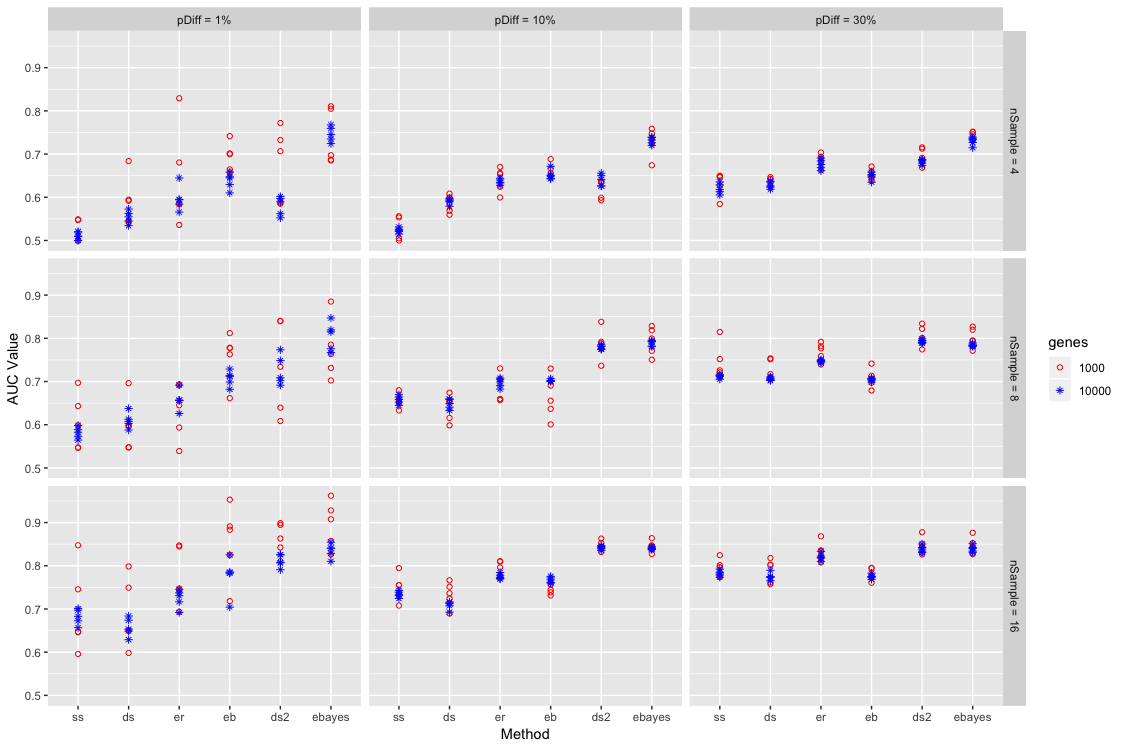
\includegraphics[scale=0.4]{auc_facet_plot}
\caption{Facet AUC Plot}
\label{auc}
\end{figure}

In terms of AUC values, ebayes method always have promising DE analysis performance.

When number of samples increases, AUC values of all methods increase. 

When DE proportion increases, the difference among the methods decreases. 

There is no obvious difference when number of genes differ.











\section{Simulation study based on a maize experiment}

To assess the efficacy of ebayes method to identify genes demonstrating DE, I used a maize dataset with two varieties B73 and Mo17\citep{paschold2012complementation} to determine realistic parameter values for a simulation study.I compared ebayes method to approaches using the R packages {\tt sSeq, DESeq, edgeR, EBSeq, and DESeq2}.

I used ebayes method to obtain normalization factors $\hat{\gamma}$ and gene-specific parameter estimates $\hat{\theta}_g$ for all genes using the {\tt edgeR} package\citep{robinson2010edger} applied to the maize data\citep{paschold2012complementation} on $27619$ genes with average count at least one and at most two zeros read counts for each variety across all the replicates. This analysis produced sample-specific normalization factors of $\hat{\gamma} = (0.923, 0.932, 1.029, 1.022, 0.973, 0.972, 1.063, 1.098)$. The gene-specific parameter estimates were treated as the true parameter values for the simulation study so that my simulated datasets mimicked the existing structure among the gene-variety means of the original maize data.

Using these parameters and normalization factors, I simulated data according to the negative binomial model in equation \ref{eq:1} independently for each gene, where $\exp{\psi_g}$ is the genewise dispersion calculated by Cox and Reid adjusted profile likelihood (CR-APL) method, the normalized factors $\gamma_{ij} = log(N_{ij})$, link function $\lambda_{gi} = X\beta_{gi}$, and the expected value $\mu_{gij} = \exp{(\lambda_{gi}+\gamma_{ij})} = N_{ij} \times \exp{(X\beta_{gi})}$. In the GLM setting, the mean response $\mu_{gij}$ is linked to a linear predictor with the base $e$ logarithm link according to equation \ref{eq:7}

\begin{equation}
\label{eq:7}
log(\mu_{gij}) = \lambda_{gi}+\gamma_{ij} = X\beta_{gi} + log(N_{ij})
\end{equation}

where $X$ is the design matrix containing the covariates (varieties), $\beta_g$ is a vector of regression parameters, and $N_{ij}$ is the effective library size for variety $i$ replicate $j$.

For each simulation, I analyzed a subset of $nGenes=1000$ or $nGenes=10000$ selected randomly from original maize count data. The library size of each sample in a simulated dataset was generated from a uniform distribution whose parameters were estimated from the maximum and minimum of the original maize count data. I repeated the simulation 5 times for each of 2, 4, and 8 replicates per variety, each of $1\%, 10\%, 30\%$ differentiation expression proportions, reusing normalization factors. 

Given the parameters gene-specific parameter estimates $\hat{\theta}_g$, I set up the simulation scenarios as the following table \ref{tab:Scenario}:

\begin{table}[H]
\centering
\begin{tabular}{|r|r|r|r|r|}
\hline
sc & nGenes & nSamples & pDiff \\ 
\hline
1 & 10000 & 8 & 0.10 \\ 
\hline
2 & 10000 & 8 & 0.30 \\ 
\hline
3 & 10000 & 8 & 0.01 \\
\hline
4 & 10000 & 4 & 0.10 \\
\hline
5 & 10000 & 4 & 0.30 \\
\hline
6 & 10000 & 4 & 0.01 \\ 
\hline
7 & 10000 & 16 & 0.10 \\
\hline
8 & 10000 & 16 & 0.30 \\ 
\hline
9 & 10000 & 16 & 0.01 \\
\hline
10& 1000 & 8 & 0.10 \\
\hline
11 & 1000 & 8 & 0.30 \\
\hline
12 & 1000 & 8 & 0.01 \\ 
\hline
13 & 1000 & 4 & 0.10 \\
\hline
14 & 1000 & 4 & 0.30 \\
\hline
15 & 1000 & 4 & 0.01 \\ 
\hline
16 & 1000 & 16 & 0.10 \\
\hline
17 & 1000 & 16 & 0.30 \\ 
\hline
18 & 1000 & 16 & 0.01 \\ 
\hline
\end{tabular}
\caption{Simulation Scenario Table}
\label{tab:Scenario}
\end{table}

For a particular gene, the truth was determined via the proportion of differential gene expression (pDiff) in the scenario setup. I randomly selected $nGenes \times (1-pDiff)$ genes and assign the expected variety count means the same as $\mu_{g1} = \mu_{g2} = 1/(n_1+n_2)\times \sum_{i=1}^2 \sum_{j=1}^{n_i} Y_{gij}$ for the selected non-DE genes. 